\begin{flushright} {\tiny {\color{gray} \tt pair\_qqq.tex}} \end{flushright}
%~~~~~~~~~~~~~~~~~~~~~~~~~~~~~~~~~~~~~~~~~~~~~~~~~~~~~~~~~~~~~~~~~~~~~~~~~~~~~~~~~~~~~~~~~~~~~~~~~~

This element pair is introduced in \textcite{zhan09} (2009) where it is 
shown to be stable for $k\ge 2$ (along with optimal order of convergence). 
Then in \textcite{huzh11} (2011) it is 
shown to be stable for $k\ge 1$. 
Note that in both cases the pressure space is the space of discontinuous 
polynomials fo separated degree $k$ or less, {\it with spurious modes filtered}.
To be precise, $Q_k^-$ is the divergence of the discrete velocity space $Q_{k+1,k}\times Q_{k,k+1}$.
The author states:
\begin{displayquote}
{\color{darkgray}
This is the first divergence-free element found on nontriangular grids. }
\end{displayquote}
We also read
\begin{displayquote}
{\color{darkgray}
The maximal possible (in space dimension) discrete pressure space
is the divergence of the discrete velocity space.
If so, the discrete solution for the
velocity would be also divergence-free.
[...]
to find a divergence-free element on rectangular grids, we seek a finite element space
whose divergence would be on to the discontinuous $Q_k$ space. This leads to the new
element, approximating the velocity by continuous $Q_{k+1,k}\times Q_{k,k+1}$ polynomials while
approximating the pressure by discontinuous polynomials $Q_k^- = div(Q_{k+1,k}\times Q_{k,k+1} )$
(see eq(2.4) below for the precise definition where $Q_k^- = P_h$ ).
We note that, by choosing $div(Q_{k+1,k}\times Q_{k,k+1})$ as the discrete finite element space for the pressure, the spurious
modes in discontinuous $Q_k$ space are filtered out automatically. On the other side,
the discrete velocity is divergence-free if and only if the discrete pressure space is
the divergence of the discrete velocity space. Because the divergence of a $Q_{k+1,k} \times Q_{k,k+1}$ 
polynomial is a $Q_k$ polynomial, the new element makes a perfect match for
the two discrete spaces and produces divergence-free solutions for the velocity.
}
\end{displayquote}



In the 2011 paper we find the following enlightening figure for $Q_{21}\times Q_{12}\times Q_1^-$:
\begin{center}
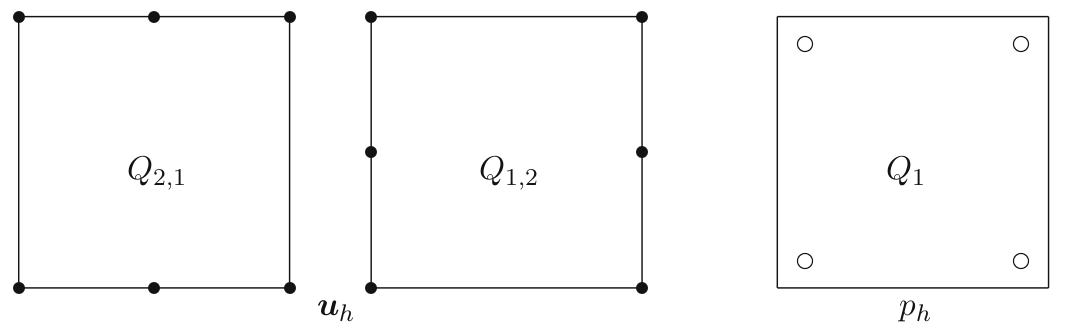
\includegraphics[width=8cm]{images/pair_qqq/huzh11}
\end{center}
and we read
\begin{displayquote}
{\color{darkgray}
The velocity
space is the continuous $Q_{2,1}\times Q_{1,2}$ space, i.e., the first component of velocity
is a piecewise polynomial of degree 2 in $x$ direction but degree 1 in $y$ direction
while the second component is a rotation of the first one. The pressure space
is the subspace of discontinuous bilinear polynomials, the divergence of the
velocity, to be explicit.
[...]
we decrease the space $Q_1^{dc}$ for the pressure to $Q_1'$ , by removing all spurious modes, i.e.,
eliminating one degree of freedom at each vertex.
}
\end{displayquote}
I do not understand the second statement (yet).


The $u$-space basis functions are given by 
\[
\vec\bN_u = Q_2 \times Q_1 =
\left(
\begin{array}{c}
\frac12 r(r-1) \\
1-r^2 \\
\frac12 r(r+1)
\end{array}
\right)
\times
\left(
\frac12 (1-s) \qquad \frac12(1+s)
\right)
=
\left(
\begin{array}{c}
\frac12 r(r-1)  \frac12(1-s)\\ 
(1-r^2)         \frac12(1-s)\\
\frac12 r(r+1)  \frac12(1-s)\\
\frac12 r(r-1)  \frac12(1+s)\\
(1-r^2)         \frac12(1+s)\\
\frac12 r(r+1)  \frac12(1+s)
\end{array}
\right)
=
\left(
\begin{array}{c}
\bN_1^u \\ 
\bN_2^u \\ 
\bN_3^u \\ 
\bN_4^u \\ 
\bN_5^u \\ 
\bN_6^u 
\end{array}
\right)
\]

\[
\vec\bN_v = Q_1 \times Q_2 = 
\left(
\begin{array}{c}
\frac12 (1-r) \\
\frac12(1+r)
\end{array}
\right)
\times
\left(
\frac12 s(s-1)  \quad
1-s^2 \quad
\frac12 s(s+1)
\right)
=
\left(
\begin{array}{c}
\frac12 (1-r) \frac12 s(s-1) \\
\frac12(1+r)  \frac12 s(s-1) \\
\frac12 (1-r) (1-s^2) \\
\frac12(1+r)  (1-s^2) \\
\frac12 (1-r) \frac12 s(s+1)\\
\frac12(1+r)  \frac12 s(s+1)
\end{array}
\right)
=
\left(
\begin{array}{c}
\bN_1^v \\ 
\bN_2^v \\ 
\bN_3^v \\ 
\bN_4^v \\ 
\bN_5^v \\ 
\bN_6^v 
\end{array}
\right)
\]
The $u$-dofs and $v$-dofs are living on different nodes.
Based on the vectors above the numbering is then 
\begin{verbatim}
4===5===6   5=======6   4=======3
|       |   |       |   |       |
|       |   3       4   |       |
|       |   |       |   |       |
1===2===3   1=======2   1=======2

 u dofs      v dofs       p dofs

\end{verbatim}
In total, there are 6 $u$-dofs, 6 $v$-dofs and 4 $p$-dofs per element.


The solution strategy is also quite peculiar (and identical to both papers, but 
following quote taken from \cite{huzh11}):
\begin{displayquote}
{\color{darkgray}
We have to emphasize
that the discrete pressure space is introduced for the analysis, but not in the
computation. By an iterated penalty method, we obtain the discrete solutions
for the pressure without coding the pressure element, as the pressure
solution is a byproduct, cf. [30] and Section 4 below. This is an advantage
of the divergence-free element, which is not carried to other mixed-finite
elements, neither to nonconforming (discontinuous) locally-divergence-free
elements [6,10,12,14,15,17,28].
}
\end{displayquote}

Reading further, we find:
\begin{displayquote}
{\color{darkgray}
It is apparent that the discrete velocity solution is divergence-free if and only if the
discrete pressure finite element space is the divergence of the discrete velocity
finite element space.
We note that by (2.4), $P_h$ is a subspace of discontinuous, piecewise bilinear
polynomials. As singular vertices are present (see [23,24]), $P_h$ is a proper subset
of the discontinuous piecewise $Q_1$ polynomials. It is possible, but difficult to
find a local basis for $P_h$. However, on the other side, it is the special interest
of the divergence-free finite element method that the space $P_h$ can be omitted
in computation and the discrete solutions approximating the pressure function
in the Stokes equations can be obtained as byproducts, if an iterated penalty
method is adopted to solve system (2.5).
}
\end{displayquote}

\begin{center}
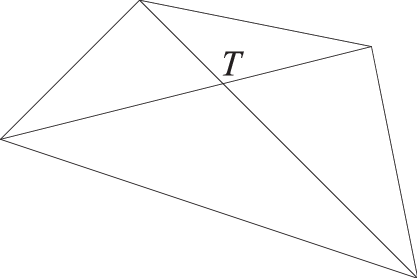
\includegraphics[width=4cm]{images/pair_qqq/singular}\\
{\captionfont ``A 2D vertex
of a triangulation is singular if all edges meeting at the vertex form two cross 
lines \cite{zhan11a}}
\end{center}

The iterated penalty method is described (for now) in \stone~161 where the 
second order version of this element is implemented.




Turning now to $Q_{3,2}\times Q_{2,3}\times Q_{2}$
\begin{verbatim}
9=10=11=12   10=11==12   7===8===9
|        |   |       |   |       |
|        |   7   8   9   |       |
5==6==7==8   |       |   4   5   6
|        |   4   5   6   |       |
|        |   |       |   |       |
1==2==3==4   1===2===3   1===2===3

 u dofs      v dofs       p dofs

\end{verbatim}
In total, there are 12 $u$-dofs, 12 $v$-dofs and 9 $p$-dofs per element.

The $u$-space basis functions are given by 
\[
\vec\bN_u = Q_3 \times Q_2 =
\left(
\begin{array}{c}
\frac{1}{16} (-1+  r+9r^2- 9r^3 ) \\
\frac{1}{16} ( 9-27r-9r^2+27r^3 ) \\
\frac{1}{16} ( 9+27r-9r^2-27r^3 ) \\
\frac{1}{16} (-1-  r+9r^2+ 9r^3 ) 
\end{array}
\right)
\times
\left(
\frac12 s(s-1)  \quad
1-s^2 \quad
\frac12 s(s+1)
\right)
\]
The other basis functions follow simply from this. Same for $Q_{4,3}$ and $Q_{3,4}$.


Open questions:
\begin{itemize}
\item 3D is discussed in \cite{zhan09} (2009) for $k\ge 2$ but quid of 3D for $k=1$? (not discussed in 2011 paper) 
\item quid of deformed elements?
\end{itemize}




